
Um motor DC é basicamente uma máquina elétrica de corrente contínua, que converte energia elétrica de corrente contínua em energia mecânica
Máquinas elétricas CC são mais fácies de controlar e oferecem uma grande faixa de velocidades \cite{Maquinas_eletricas}.
Devido a sua facilidade de controle, se tornam ótimos canditados para uso em eletrónica e robótica, pois podem ser usados com baterias
Para controlar a velocidade de um motor, é necessário o uso de um encoder, que converte o sinal de posição em um valor medível de velocidade angular.


O motor a ser usado será um motor DC de 6V 210rpm, com taxa de redução de 1:34
O encoder a ser usado nesse projeto é um encoder magnético, que já vem montado no motor a ser usado, com 11 PPR (Pulses Per Revolution).

\subsection{Encoder magnético}

Por ser um encoder PRR, ele produz duas ondas quadradas como saídas, A e B \cite{encoder_ppr}.
As duas possui 90° de fase em si, e se a onda A estiver adiantada em relação a onda B (\ref{encoder_ppr_ab}), o sentido de rotação é positivo (contra o relógio)

\begin{figure}[h]
	\centering
	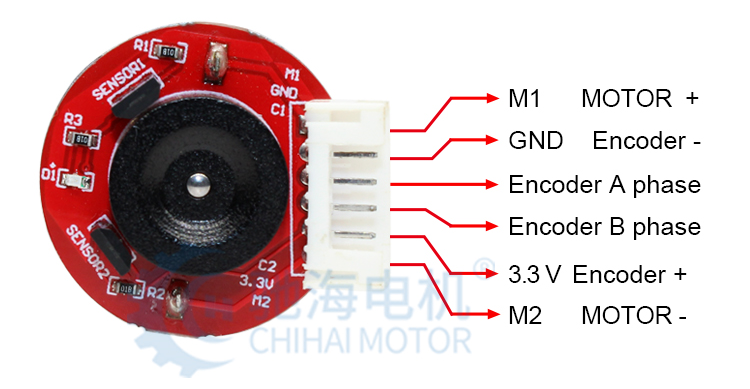
\includegraphics[width=0.6\textwidth]{figures/encoder_holzer}
	\caption{Encoder holzer \cite{encoder_holzer}}
\end{figure}

\begin{figure}[h]
	\centering
	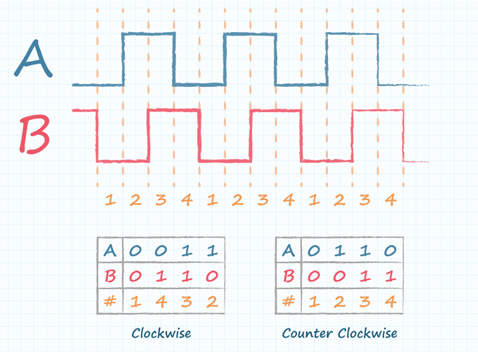
\includegraphics[width=0.7\textwidth]{figures/encoder_pulso_ab}
	\caption{Ondas quadradas resultantes dos pulsos de saída do encoder \cite{encoder_ppr}}
	\label{encoder_ppr_ab}
\end{figure}


